\begin{figure*}[!th]
\centering
% \includegraphics[width=\textwidth]{./images/Tech_Details_Transformer.pdf}
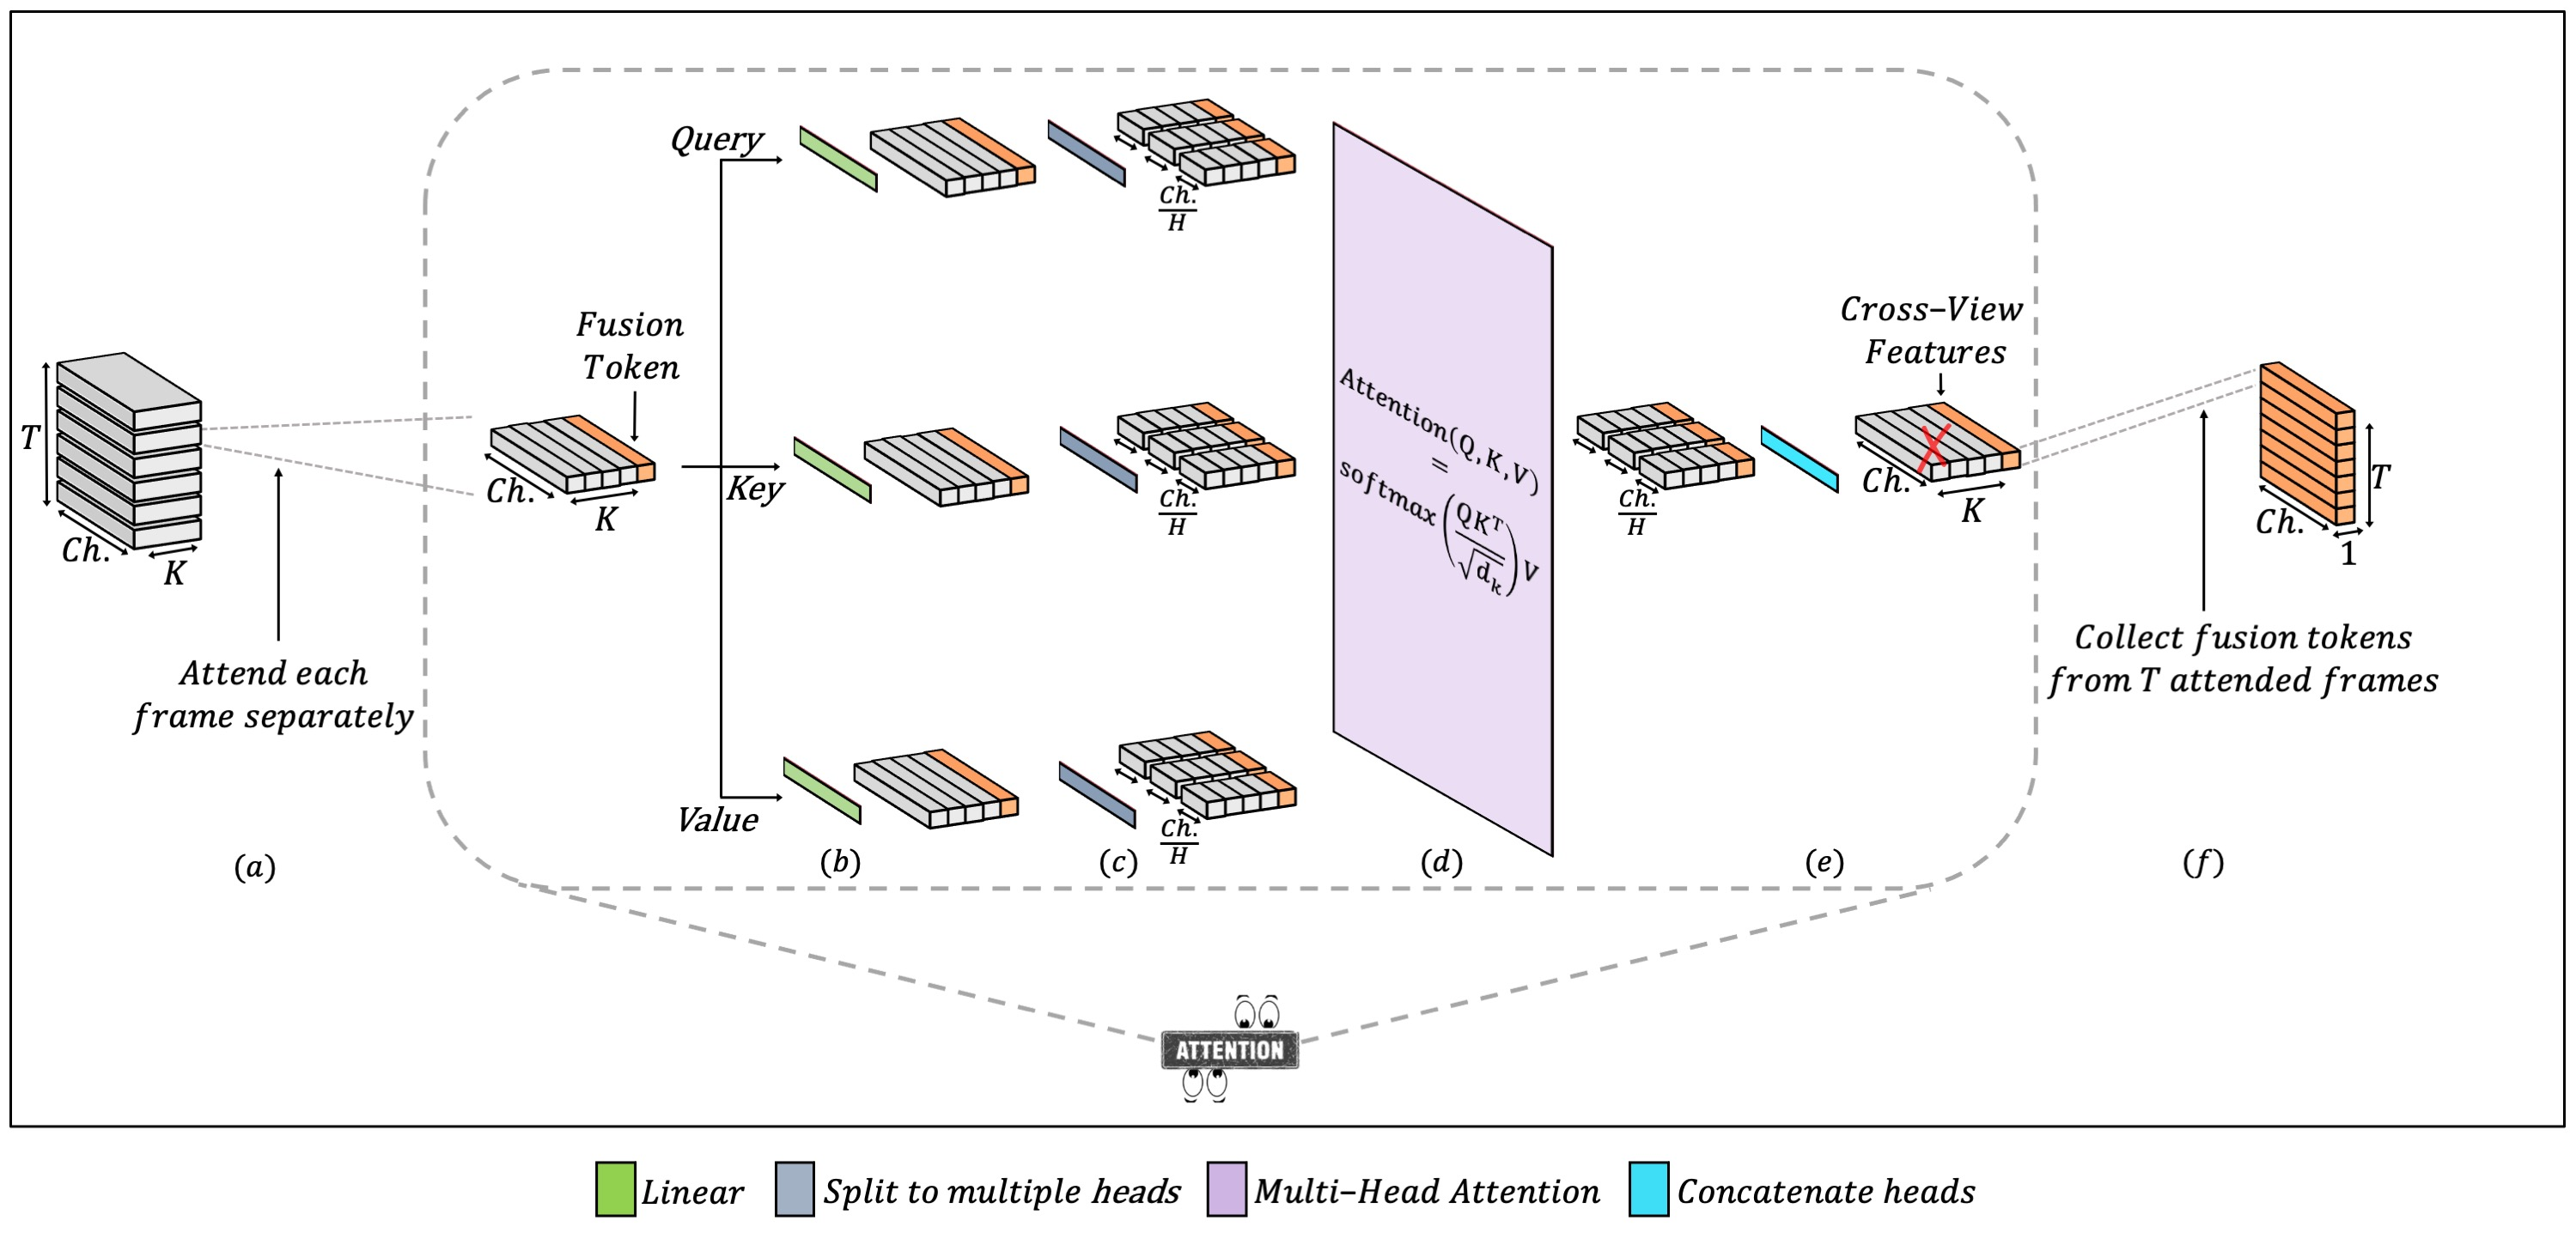
\includegraphics[width=\linewidth]{./images/Attention_diagram.jpg}

\setlength{\abovecaptionskip}{5pt plus 3pt minus 2pt}
\setlength{\belowcaptionskip}{-10pt plus 3pt minus 2pt}
\caption{\bg{Cross-view attention layer (\Cref{fig:architecture_detail}(d)) in detail. Our attention mechanism processes each frame separately, attending the multi-view features and fusing them to a single output per frame. 
(a)~Process each temporal frame independently. Add a learned token~\cite{BERT} that forms a \emph{fusion view}; 
%A learned fusion token is added to multi-view .... , similar approach as Devlin~\etal\cite{BERT}; 
(b)~Linear layer; 
(c)~Split the channels to $H$ attention heads; 
(d)~Multi-Head attention~\cite{attn_is_all_you_need}; 
(e)~Concatenate the attention heads; 
(f)~Drop features from the original views. Collect fusion view features from all the frames in the temporal sequence. }}
\label{fig:attention_detail}
\end{figure*}